\documentclass[a4paper]{report}

\usepackage[utf8]{inputenc}
\usepackage[T1]{fontenc}
\usepackage[francais]{babel}

\usepackage{graphicx}

\title{Extraction de connaissance dans les données\\Projet de classification de documents par opinion}
\author{Mehdi BENNIS -- Thibaut ETIENNE -- Fabien FERAUD\\Florian NOVELLON -- Arnaud SOULIER}

\begin{document}
    \maketitle

    \newpage
    \null
    \newpage

    \tableofcontents
    \newpage

    \chapter{Introduction}

        Dans le cadre de notre formation du second semestre M1 et dans l’UE HMIN208 - Extraction des connaissances dans les données, on a été amené à réaliser un projet qui consiste à analyser une liste volumineuse de données représentante des avis d’internautes sur des films, où chaque avis a sa polarité (+1 s’il est positif, -1 s’il est négatif).

        Pour traiter ces données, un choix s’est présenté sur le langage a utilisé (Java, Python, Php, R) ainsi que sur la technologie de classification, Weka, Scikit learn ou R.

        Notre choix de langage s’est vite orienté vers python vu sa simplicité d’implémentation et l’engouement du groupe vis-à-vis de ce langage.
        En ce qui concerne la technologie de classification choisie, Scikit learn a été un choix rapide vu que c’est une bibliothèque libre Python.

        La réalisation du projet consistait à expérimenter différents algorithmes de classification, analyser les résultats obtenus, les comparer et ceci par le biais de 4 étapes dirigées par l’énoncé fourni par nos encadrants.

        Lors de la réalisation du projet, un challenge a été lancé. Il consistait à analyser un nouveau jeu de données et prédire leur polarité sans connaître la réponse. Pour cela, il fallait utiliser les programmes implémenter en fonction de nos choix de pré-traitement et de classifier déterminé grâce au premier jeu de données de test. Ce challenge avait pour but de vérifier si nos choix étaient les bons.

    \chapter{Pré-traitement}

        \section{Tokenisation}

            La première étape que nous avons choisie pour pré-traiter les textes est d'en séparer chacun des mots.
            Pour cela, nous avons décidé d'utiliser la fonction tokenize de la librairie ntlk. Elle retourne une liste de mots à partir d'une chaîne de caractères.

            Avec cette liste de mots nous pourrons facilement appliquer chaque traitement sur les mots indépendamment les uns des autres.

            Durant cette phase, nous corrigeons également des erreurs de syntaxe telles que les points de fin de phrase qui restent collés aux mots. Nous les recherchons et les séparons pour éviter d'avoir deux mots dans un token.

            Exemple :
            “Hello world, i’m a python” $\rightarrow$ [“Hello”, ”world”, ”i”, ” ’ ”, ”m”, ”a”, ”python”].

        \section{Minuscule}

            L’étape précédente se base sur la casse des mots pour corriger quelques erreurs syntaxiques. Il est en effet important d’avoir des données les plus propres possible. Maintenant que ce problème a été réglé au mieux, la casse des mots ne nous apporte plus aucune information, au contraire elle nous en fait perdre.

            En effet, si tous les algorithmes que l’on doit appliquer doivent tenir compte de la casse des mots, les traitements seraient bien plus lourds donc plus longs. De ce fait, on formate les données ( dans notre cas nos opinions) pour que tout soit en lettre minuscule.

            On obtient le même résultat que si on avait gardé la casse mais les algorithmes deviennent plus rapides car ils savent que toutes les données sont en minuscules.

        \section{Tree Tagger}

            L’installation du TreeTaggerWrapper nécessite l’utilisation du TreeTagger qui est libre d’accès seulement pour des buts éducatifs et de recherches. Après avoir installé le TreeTagger l’installation du TreeTaggerWrapper est simpliste via la commande ‘pip’ et est fonctionnelle correctement en Python2 et 3.

            \subsection{Fonctionnement}

                Le fonctionnement basique du TreeTaggerWrapper est une fonction qui prend un texte en entrée telle une chaîne de caractères ou un texte, et ce dernier renvoie ce même texte lemmatisé et avec chaque mot son tag correspondant. (Ex : [JJ] pour adjectif, [NN] Nom, ...).

                Ce résultat est utilisé pour enlever les types de mots que nous estimons inutiles pour définir la polarité des opinions.

            \subsection{Choix des tags}

                Notre choix de tag s’est fait de manière à joindre l’intuition linguistique et l’expérimentation pour les algorithmes utilisés dans notre prétraitement. Puis analyser les différents résultats, les comparer et refaire des choix en conséquences.
                Les tags les plus importants qui impactent énormément le résultat sont les Adjectifs et les Adjectifs de comparaison ou ce qui permet de décrire toute autre polarité positive ou négative.

                L’un des meilleurs résultats obtenus est le suivant (les mots tagués à retirer) : ["CC", "DT", "EX", "FW", "IN", "IN/that", "LS", "MD", "PDT", "POS", "PP", "PP\$", "SENT", "SYM", "TO", "UH", "WDT", "WP", "WRB", ":", "\$"]

                \begin{itemize}
                    \item CC : coordinating conjunction
                    \item DT : determiner
                    \item EX : existential there
                    \item FW : foreign word
                    \item IN : preposition/subord. conj
                    \item IN/that : complementizer
                    \item LS : list marker
                    \item MD : modal
                    \item PDT :	predeterminer
                    \item POS :	possessive ending
                    \item PP : personal pronoun
                    \item PP\$ : possessive pronoun
                    \item SENT : end punctuation
                    \item SYM : symbol
                    \item TO : to
                    \item UH : interjection
                    \item WDT : wh-determiner
                    \item WP : wh-pronoun
                    \item WRB : wh-abverb
                    \item ‘:’ : general joiner
                    \item \$ : currency symbol\\
                \end{itemize}

                \textbf{Remarque importante :}\\
                La fonctionnalité TreeTagger dispose de son propre programme de lemmatisation et ce dernier est intelligent. L’ordre des fonctions de prétraitement sont très importantes car celles-ci peuvent influer négativement comme positivement les unes sur les autres.

                Par exemple lemmatiser et enlever les stop words avant d’utiliser le TreeTagger diminue la précision du TreeTagger, car ce dernier tague mot par mot en fonction de son contexte grammatical.

                Exemple : [I watch] pronom personnel et verbe alors que [watch] (supposons le “I” retiré par les stop words) donnera un nom, une montre au lieu de regarder.

        \section{Suppression des stop-words}

            Certains mots ne seront pas intéressants à garder pour la classification. Afin d'éviter de surcharger notre texte de ces mots inutiles, nous avons construit une liste de stop-words dont les occurrences dans le texte seront supprimées. Grâce à la conversion en minuscules et les corrections de syntaxe décrites précédemment, aucun mot ne sera oublié.

            La construction de cette liste s’est faite en plusieurs temps :
            \begin{itemize}
                \item Au début du projet, on a utilisé une liste de stop word fourni par scikit learn. La liste était assez générale, de ce fait un travail de lecture a été opéré afin d’enlever ce qu’il semblait être inadéquat au sujet.
                \item Dans un deuxième temps, un programme python a été implémenté afin d’observer chaque mot des opinions et leur nombre d'occurrences. De cette liste, une sélection des mots avec le plus d'occurrences et n’ayant pas d’utilités pour notre cas a été extraite puis ajoutée à la liste des stop-words.
                \item Enfin la liste a été complété par une sélection parmi une liste de stop-words pour film trouvé sur internet.
            \end{itemize}

            Au fur et à mesure des tests cette liste a été modifiée pour être la plus optimale pour notre problématique.

        \section{Lemmatisation}

        La lemmatisation est une opération permettant de simplifier la syntaxe des mots en échangeant, par exemple, les verbes conjugués par leur infinitif ou les noms pluriels par leur singulier.

        Cette opération permet de limiter la diversité des mots et garder un mot précis pour exprimer un avis précis.

        Plus précisément, un mot peut apparaître dans un texte sous plusieurs formes, conjugué, participe passé, pluriel, etc. Ces mêmes formes retrouvent tous leur forme d’origine appelée Lemma qui était le mot de base.

        Exemple : ‘Walk’, ‘Walks’, ‘Walking’,’Walked’ : leur lemmatisation donne ‘Walk’ comme Lemma.

    \chapter{Cross-validation}

        \section{Fonctionnement}

            La cross-validation (validation croisée) est une méthode aidant la validation d’un modèle grâce à une technique d’estimation de fiabilité de celui-ci.
            Le principe est d’échantillonner les données d'entraînement K fois. Pour chaque échantillon une partie des données est utilisée pour l'entraînement du classifieur et l’autre partie pour tester son efficacité (voir Figure \ref{fig:1}).

            \begin{figure}
                \centering
                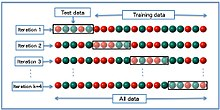
\includegraphics[width=.6\linewidth]{cross_validation.png}
                \caption{Illustration d’un échantillonnage pour K = 4}
                \label{fig:1}
            \end{figure}

            Suite à ces K tests, on obtient K résultats d’efficacités sur lesquels on calcule la moyenne et l’écart entre le minimum et le maximum.
            La moyenne nous permet de savoir si notre modèle est efficace, cependant cette donnée seule ne nous révèle pas si le modèle est fiable.

            Par exemple prenons un cross-validate avec K = 5 nous donnant les F-mesures suivantes : [ 0.95, 0.65, 0.85, 0.90, 0.90 ].
            On obtient une moyenne de 0.85, ce qui est assez haut. Cependant l’écart entre le minimum et la maximum est de 0.3 ce qui est assez grand aussi. On peut en conclure que ce modèle est efficace dans la plupart des cas mais n’est pas vraiment très fiable.

            On peut donc dire qu’un modèle est valide lorsque les résultats de notre cross-validation nous donnent une moyenne la plus haute possible tout en gardant un écart entre la f-mesure maximum et la f-mesure minimum le plus bas possible.

        \section{Analyse de nos résultats}



    \chapter{Analyse des résultats}



    \chapter{Challenge}

        Les résultats du challenge ont été décevants. Les tests effectués avec les pré-traitements et les classifieurs implémentés sur les données d'entraînements donnaient un résultat en moyenne de 0.87 soit 87\% de bonnes estimations.

        Or lorsque les résultats du challenge sortent, le résultat est de 0.494. La moitié de nos résultats sont corrects.

        Étonnés par ces résultats, nous avons analysé notre code. Nous nous sommes rendu compte que la méthode que l’on utilisait pour séparer nos données faisait en premier un mélange puis les découpait en un morceau d’apprentissage et un morceau de prédiction. Pour les données d'entraînement, cela était parfait car elles étaient ordonnées et cela mélangeait de la même manière le fichier contenant les labels des données d’entrainements.

        Quand on a voulu appliquer notre programme avec un apprentissage sur toutes les données d’apprentissages et la prédiction sur les données du challenge, on a utilisé la même méthode en modifiant la séparation pour l’apprentissage et pour la prédiction.

        Le souci est que la méthode a mélangé les données du challenge puis a prédit dessus. La vérification a été faussée car la comparaison entre le premier résultat de notre fichier correspondant par exemple à l’avis 254 à cause du mélange et le premier résultat des données du challenge étant celui de l’avis 1.

        Notre programme avait donc prédit correctement, comme on a pu le voir une fois le problème du mélange réglé on a dépassé les 90\% de réussite.

    \chapter{Gestion de projet}

        

    \chapter{Conclusion}

        Ce projet nous a permis de comprendre avec précision comment fonctionne le machine learning. La liberté du choix du langage et la liberté des choix au niveau des classifieurs et du traitement du texte ont été intéressantes. Nous avons pu réaliser de nombreux tests pour déterminer quel classifieur couplé à quel traitement du texte nous donnera le meilleur résultat possible.

        Notre erreur pour le challenge nous a permis de clarifier le code pour trouver d’où venait l’erreur. De plus, c’est en cherchant des réponses à notre problème que l’on a trouvé la cross-validation. On a alors automatisé nos tests afin d’implémenter cette cross-validation et de trouver la meilleure méthode pour le challenge. Ce concept de validation croisée nous manqué et cela nous a permis de le découvrir.

        Nous avons donc obtenu le résultat suivant : l’algorithme (classifieur) nous donnant le meilleur résultat est le Support Vector Classification (SVC) avec 0,931 (93,1\%) au challenge mais néanmoins il nécessite un temps d'exécution très important (environ 40 minutes).
        Nous pouvons donc dire que le classifieur Naïve Bayes nous donne des résultats très convenables (0,91 (91\%)) pour sa durée d’exécution d’environ dix secondes

        L’amélioration de nos résultats est probablement possible, par exemple pour certains classifieurs comme NB, le choix des stop words à supprimer ou encore le choix des tree tagger à supprimer peut modifier en bien nos résultats mais nécessiterait de très nombreux tests.

\end{document}
